\chapter{Estudo de Caso}
\label{ap:elastic}

\section{E-Lastic}
O E-lastic é um sistema eletrônico que monitora e controla a execução de exercícios físicos realizados com equipamento que impõe sobrecarga à movimentação de segmentos corporais por meio de resistência elástica. Geralmente o controle de sobrecarga gerada por elementos elásticos é baseado na percepção subjetiva do esforço, com base na sensação de fadiga experimentada durante o exercício, e portanto o praticante não têm controle do esforço aplicado no exercício.

O produto em desenvolvimento apresenta um aparelho portátil, voltado para o controle de atividades físicas em ambientes fechados ou abertos. Trata-se de um sistema eletrônico embarcado que realiza o processamento digital do sinal originado num sensor de força e associa essas informações com variáveis de espaço e tempo, de forma a gerar informações suficientes para o controle e prescrição de exercícios resistidos. O sensor de força será fornecido calibrado juntamente com a central de processamento. Esse sistema eletrônico permite a acoplagem do implemento elástico para a realização do exercício a ser monitorado, e interfaceia com o usuário por meio de um aplicativo desenvolvido para um dispositivo móvel. De forma simplificada, durante o exercício físico, a força aplicada pelo usuário ao elemento elástico é calculada no microcontrolador e enviada juntamente com as demais informações via \textit{Bluetooth} para um dispositivo móvel com o e-lastic \textit{app}, que contém opções de controle para a realização do exercício físico.

Para a utilização do aparelho, o usuário deve selecionar o implemento elástico mais adequado ao exercício que será praticado, com resistência elástica compatível com o esforço que será aplicado. Um sensor de força compatível é acoplado ao implemento elástico e ligado ao módulo de processamento por uma entrada específica. O usuário então seleciona via aplicativo móvel um dos três modos de execução de exercício: dinâmico, isométrico e potência. Seleciona em seguida a configuração da sua rotina de treino, com os parâmetros de controle para o exercício específico. A partir daí o exercício pode ser iniciado, e informações precisas de controle são apresentadas na tela do dispositivo móvel em tempo real. Vibração do dispositivo, estímulos sonoros e outros tipos de sinais podem ser utilizados para dar \textit{biofeedback} ao usuário sobre o exercício em curso. Após a realização do exercício, é apresentado um resumo da seção de treino executada. É possível que se apresente um histórico de treinamento dos indivíduos que realizam suas atividades utilizando o e-lastic.

Os parâmetros para controle podem variar de exercício para exercício, porém em todos eles será selecionado um intervalo de intensidade, isto é, carga máxima e mínima em quilogramas, em que o exercício será trabalhado. As opções de exercícios são espécies de rotinas pré programadas, modos de utilização da resistência elástica para o exercício físico:

\begin{enumerate}
\item Modo dinâmico - Realização de movimentos cíclicos em velocidade lenta e cadência controlada. Os parâmetros de controle para esse exercício são número de séries de exercícios, número de repetições por série e a duração do descanso entre as séries.
\item Modo isométrico - Contrações estáticas em que o usuário mantém uma posição e sustenta a sobrecarga elástica nessa posição por um determinado tempo. Semelhante ao modo dinâmico, no modo isométrico o usuário seleciona os parâmetros de números de contrações realizadas (repetições do exercício), e duração do tempo de intervalo entre as séries, com adição da duração de cada contração, isto é, o tempo em que o esforço deve ser mantido para que uma repetição seja contabilizada.
\item Modo potência - Semelhante ao modo dinâmico, estes são exercícios cíclicos, porém com a maior velocidade possível. Os parâmetros para esse exercício são os mesmos do modo dinâmico, porém aqui a velocidade do movimento faz parte dos parâmetros de controle.
\end{enumerate}

\section{Desenvolvimento}

O e-lastic começou como um produto desenvolvido para interfacear com usuário por modo de um dispositivo específico conectado ao sensor de força via cabo. A seleção dos exercícios e o próprio \textit{feedback} para o usuário eram realizados por meio desse dispositivo, fazendo interação com o usuário por meio de um display LCD e um potenciômetro para seleção de parâmetros de exercício, e o \textit{feedback} sendo feito por meio de LEDs e sinais sonoros, bem como o próprio display LCD. Esse produto é resultado do trabalho de mestrado em processamento de sinais da aluna Fernanda Sampaio Teles, que resultou num pedido de patente com número de registro BR 5120130007631.

Por volta de 1 vez ao mês, foram realizadas reuniões com Fernanda e outros integrantes da equipe. Daqui em diante serão referenciados neste documento como \textit{product owners}.

Os requisitos para o aplicativo foram a principio retirados do próprio comportamento dos primeiros protótipos. Esses comportamentos foram descritos e detalhados pelos \textit{product owners}, que não só descreveram como os protótipos funcionavam, como também foi discutido como o aplicativo deveria se comportar de forma diferente dos mesmos, com adições de novas funcionalidades para o aplicativo sendo desenvolvido.

A ideia inicial do aplicativo, e foco principal do desenvolvimento da equipe ao longo desse semestre, foi fazer com que o aplicativo sendo desenvolvido para plataforma Android tenha no mínimo as mesmas funcionalidades dos primeiros protótipos. 

O desenvolvimento do e-lastic app ao longo do semestre foi planejado e executado juntamente com a disciplina de Manutenção e Evolução de Software (MES). Desde o início do semestre, foi preparada uma equipe na disciplina para o desenvolvimento do aplicativo desde o início, de forma a preparar a base da arquitetura. Essa base será utilizada na segunda fase deste trabalho, quando o desenvolvimento será focado em alcançar todos os objetivos traçados nas reuniões com os \textit{product owners}, que se resumem basicamente na construção e entrega do aplicativo completo e funcional.

Para este trabalho em conjunto com a disciplina de MES durante o semestre, o objetivo principal é conseguir uma base de arquitetura e alcançar dois tipos de exercícios com funcionalidade implementada: exercício dinâmico e isométrico. A interface gráfica foi deixada em segundo plano durante esse período de desenvolvimento, com o foco voltado então em uma base estável e manutenível com as funcionalidades básicas implementadas e com seus respectivos testes.

\subsection{Ciclo de desenvolvimento}		

Durante o desenvolvimento, foram utilizadas práticas ágeis retiradas do Scrum. Embora o Scrum não esteja no escopo deste trabalho, informações sobre o mesmo podem ser obtidas em \citeonline{scrum}.

Devido ao ritmo de trabalho mais lento proporcionado pelo tempo curto da disciplina de MES, as \textit{sprints} foram planejadas para durar 15 dias (2 semanas). Inicialmente foram criadas várias histórias de usuário (\textit{user stories}) e montado um \textit{backlog} considerando a reunião inicial com os \textit{product owners}. Novas histórias surgiam, bem como histórias iam sendo atualizadas conforme os requisitos ficavam mais claros com as reuniões subsequentes. A cada 2 semanas então eram consideradas as histórias de usuário do \textit{backlog} e priorizadas para a iniciar a \textit{sprint}. Nas medidas utilizadas pela equipe, com pontuação de 1 a 5 para cada história utilizando técnica do \textit{planning poker}, foi implementada uma média de 7 \textit{story points} por \textit{sprint}. É importante ressaltar que histórias não completadas não entram nem parcialmente nesse cálculo e são jogadas para as \textit{sprints} seguintes, e portanto para uma equipe inexperiente em constante aprendizado é possível inferir que mais esforço foi dedicado do que o próprio \textit{velocity} pode indicar, representando a curva de aprendizado da equipe. Muito do esforço do principal autor deste trabalho foi direcionado ao aprendizado da equipe para alavancar o desenvolvimento do aplicativo.

Todo trabalho realizado foi feito utilizando técnica de programação em pares. Um quadro mapeando os integrantes que já trabalharam juntos esteve em constante atualização para que a equipe circulasse da melhor forma possível. O principal autor deste trabalho participou do desenvolvimento dessa forma várias vezes ao longo do semestre, mesmo esse não sendo o objetivo principal, com o intuito de compartilhar de parte do conhecimento da plataforma obtido em projeto com parceria UnB-Positivo de desenvolvimento de aplicativos Android, bem como conhecimento adquirido em estágio no ICRI-SC (\textit{Intel Collaborative Research Institute for Security Computing}), focado em segurança móvel.

O código sendo desenvolvido se encontra disponível em um repositório aberto\footnote{\url{http://gitlab.com/biodyn/biodynapp}} para qualquer desenvolvedor através da plataforma gitlab.com, e a equipe de alunos de MES não tem acesso direto de escrita para esse repositório. Para contribuir para o projeto, a equipe trabalha em uma cópia do repositório original (\textit{fork}). Quando alcança algo significativo para o projeto, a equipe então cria um \textit{merge request} pela própria plataforma gitlab, que é então avaliado e aceito pelos revisores, a exemplo do principal autor deste trabalho, ou rejeitado e mudanças são solicitadas. O mesmo procedimento pode ser realizado por qualquer desenvolvedor que deseja contribuir com o projeto. Como já dito, o software sendo desenvolvido é livre e portanto tem código aberto disponibilizado online. A única parte do produto e-lastic que será comercializada é o componente físico, com o módulo central de processamento, sensor de força e implemento elástico.

\subsection{Equipe}
Composta por 5 alunos da disciplina de MES, a equipe contém apenas graduandos em Engenharia de Software da Universidade de Brasília campus UnB Gama. Todos eles tem um tempo a dedicar ao desenvolvimento correspondente ao tempo de uma disciplina de 4 créditos, com 4 horas-aula e mais 4 horas semanais adicionais por integrante, totalizando 8 horas por semana de dedicação para cada um dos integrantes da equipe.

Todos os integrantes não tinham a priori nenhuma experiência no desenvolvimento de aplicativos para a plataforma Android, porém todos eles tinham algum conhecimento em linguagem de programação Java, necessária ao desenvolvimento, bem como experiência em atividades de verificação e validação, banco de dados, entre outras áreas. Todo esse conhecimento foi adquirido ao longo do curso de graduação em Engenharia de Software que está em andamento, provendo o background necessário para que eles pudessem trabalhar neste projeto durante o semestre. A equipe também apresentou conhecimento suficiente em gerência de configuração e controle de versionamento, o que ajudou significativamente em relação a manutenção do repositório do projeto.

Um dos integrantes da equipe faz o papel de \textit{coach}, coordenando o restante da equipe para alcançar os objetivos de cada \textit{sprint} e tomando frente da organização da equipe ao longo dos ciclos de desenvolvimento. Embora tenha essa responsabilidade adicional, esse integrante participava das atividades de desenvolvimento tanto quanto os demais, e foi selecionado para esse papel pelo professor da disciplina, orientador deste trabalho, por ter mais experiência que os demais em metodologia ágil de desenvolvimento de software.

O principal papel exercido pelo principal autor deste trabalho ao longo do desenvolvimento foi em relação ao estabelecimento da arquitetura do aplicativo sendo desenvolvido, visto que a equipe não tinha experiência com componentes do Android e não conhecia a própria estrutura de um aplicativo para essa plataforma. Dessa forma, ele ficou responsável por criar a estrutura base para o desenvolvimento do aplicativo, bem como revisar todos os códigos submetidos para o repositório principal, e solicitar modificações caso não estivessem de acordo com a arquitetura base do repositório principal, ou não estivesse com qualidade aceitável. Como o autor participou ativamente do desenvolvimento, não houve muita surpresa nos \textit{merge requests} e portanto poucos foram rejeitados.

Durante as aulas da disciplina de MES, toda a equipe esteve presente com o principal autor deste documento, onde era aproveitado o tempo em conjunto para a disseminação do conhecimento sobre a plataforma. Por várias vezes foram feitos DOJOs de treinamento para que o conhecimento circulasse dentro da equipe. Com o mesmo objetivo, a equipe sempre trabalhou em revezamento de pares e de tarefas. Uma dupla que trabalhou com um módulo específico durante uma semana passava a trabalhar em outro na semana seguinte, ou mesmo em atividades de teste, com outra dupla assumindo o trabalho da anterior. Os demais horários da equipe variam de acordo com a semana e com a dupla que trabalhará na semana. As duplas sempre alternavam, e os horários para cada dupla dependem da disponibilidade dos integrantes. Nesses horários de desenvolvimento, o autor deste trabalho não participou de forma presencial e não houve participação de toda a equipe reunida, cada dupla trabalhava em uma parte separada da aplicação.

Como os conhecimentos em desenvolvimento Android foram adquiridos ao longo do desenvolvimento, a primeira \textit{sprint} teve menor \textit{velocity} que as demais.

Embora seu principal papel fosse como arquiteto e revisor de código, o autor deste trabalho também participou da codificação do aplicativo, codificando e construindo boa parte dos principais componentes desenvolvidos ao longo do semestre. Um dos motivos para isso foi dar o impulso inicial que a equipe inexperiente na plataforma precisava para trabalhar de forma mais eficiente.

\section{Estado da Arquitetura}

O planejamento do desenvolvimento para a equipe da disciplina de MES foi focado na base da arquitetura, juntamente com a funcionalidade básica do aplicativo. Isso inclui o modo de exercício dinâmico e exercício isométrico com seus respectivos testes funcionais, e a comunicação com o microcontrolador via \textit{Bluetooth} para o funcionamento dos exercícios. A interface gráfica de usuário foi deixada em segundo plano durante essa etapa do desenvolvimento, tendo apenas alguns componentes temporários apresentados na tela para ajudar na visualização da funcionalidade que foi desenvolvida. Ainda durante esse período de colaboração com a equipe de MES, também deve ser entregue a persistência dos parâmetros de execução dos exercícios, de forma que o usuário possa salvar suas preferências e carregá-las para reutilizar os mesmo parâmetros da próxima vez que praticar o exercício.

Nesta seção, serão chamados de componentes instanciações dos componentes Android, e de módulos conjunto mais complexo de classes que envolvem um ou mais componentes. Na implementação atual do aplicativo, exitem os seguintes componentes e módulos principais:
\begin{itemize}
	\item \textit{BluetoothService} - Responsável pela conexão \textit{bluetooth}, este componente é um \textit{Android Service} que se inicia juntamente com a aplicação e fica a espera de uma solicitação de conexão vinda da tela de escolha de dispositivos. Quando o usuário solicita a conexão com o hardware e-lastic selecionando-o em uma lista, o aplicativo identifica o dispositivo a ser conectado e informa ao \textit{BluetoothService}, que a partir daí é responsável por conectar e manter a conexão, recebendo os dados do microcontrolador presente no hardware e-lastic.
	\item \textit{ExerciseService} - Este módulo reúne a maior parte da lógica de negócio. Ele gerencia qual é o exercício ativo e trata da execução do mesmo. Quando recebe um dado de força vindo do \textit{bluetoothService}, o \textit{exerciseService} informa ao exercício ativo os novos valores recebidos. Da mesma forma ele informa ao exercício sobre mudanças nos parâmetros vindas da interação com o usuário com o a tela do aplicativo.
	\item \textit{BioFeedbackService} - Este módulo é responsável por gerar \textit{biofeedback} para o usuário. Quando o valor de força é superior ao limite máximo, por exemplo, o exercício informa a esse componente que algum tipo de \textit{feedback} deve ser acionado para informar ao usuário que o limite foi ultrapassado. Por sua vez, este componente checa sua lista de \textit{biofeedbacks} e aciona os que foram solicitados. Por exemplo, pode ser solicitado que o dispositivo móvel vibre quando os limites de força forem violados, como também pode ser requisitado que um som seja tocado. Essas configurações de que tipo de \textit{biofeedback} ativar estarão disponíveis para o usuário na versão final do aplicativo.  
	\item \textit{ExerciseActivity} - Representa a tela principal e a própria interação do usuário com os componentes gráficos. Este componente não será totalmente implementado neste período de desenvolvimento com parceria com a equipe de Manutenção e Evolução de software, e será trabalhado apenas na segunda etapa deste trabalho. Neste período, apenas alguns componentes gráficos temporários estão disponíveis para demonstrar a funcionalidade básica do aplicativo em execução.
\end{itemize} 

A comunicação de todos os componentes e módulos é feita de forma indireta por meio de \textit{intents}. Como já citado em capítulos anteriores, o \textit{intent} tem a função de comunicar componentes independente da aplicação a qual pertencem. Entretanto, neste aplicativo em desenvolvimento, essa comunicação deve ser feita apenas entre os componentes internos da aplicação, não sendo necessário que esses \textit{intents} entre os componentes internos sejam enviados pelo sistema Android para outros componentes de outras aplicações. Para esse fim, a implementação foi feita utilizado um recurso da API Android chamado \textit{LocalBroadcastManager}, que é responsável por realizar o envio de \textit{broadcast intents} apenas para os componentes internos da aplicação, evitando que os mesmos sejam recebidos em outras aplicações. De forma análoga, os receptores desses \textit{intents} são registrados não diretamente no sistema, mas dentro dessa instância de \textit{LocalBroadcastManager} que é individual da aplicação, registrando-se apenas para receber \textit{intents} enviados dentro da própria aplicação. O uso desse recurso evita a necessidade de criar permissões específicas para cada tipo de \textit{intent} que será utilizado entro da aplicação, e não há perigo de que a aplicação receba \textit{intents} forjados por alguma outra aplicação maliciosa ou mesmo que alguma aplicação maliciosa receba dados que são privados deste aplicativo.

Toda essa comunicação indireta foi reunida em uma classe responsável por gerenciar essas comunicações, a classe \textit{Communicator}. Essa classe reúne todas as \textit{actions} de todos os \textit{intents} que as classes estão preparadas para receber. Basicamente, para saber que informações o \textit{ExerciseService} espera, por exemplo, basta checar as constantes na classe \textit{Communicator.ExerciseServiceActions}. Embora essa classe pareça ter um alto acoplamento devido a sua responsabilidade de comunicar todos os componentes, esse acoplamento é reduzido devido a comunicação indireta que é feita com o uso de \textit{intents}. Simplificando, a classe \textit{Communicator} tem a responsabilidade de enviar mensagens para todos os componentes sem realmente os conhecer. Se um componente for alterado, não há impacto algum dentro dessa classe.

Essa comunicação indireta que é implementada por meio dos \textit{intents} tem a vantagem de deixar os componentes com uma conexão bastante fraca. Quando um componente envia uma mensagem, ele não sabe ao certo quem vai receber, portanto não precisa conhecer o receptor. As mensagens são enviadas via \textit{broadcast}, para todos os componentes, e cada um recebe o que desejar receber. Da mesma forma, os receptores dessas mensagens não sabem quem as mandou, e portanto não há uma associação direta em nenhum dos lados da comunicação. Embora pareça deixar a comunicação confusa e embaralhada, isso permite que troquemos um componente inteiro do projeto com pequeno ou nenhum impacto nos demais componentes. A interface gráfica, por exemplo, recebe mensagens do componente de exercício informando sobre atualizações nos dados. Ela não conhece o exercício em execução e o exercício em execução não conhece quem está mostrando seus dados. Se a interface gráfica fosse inteiramente excluída da aplicação, com pouquíssimos ajustes, relacionados principalmente as mudanças no próprio \textit{AndroidManifest.xml}, seria possível deixar várias outras funcionalidades ainda em funcionamento. Com esse acoplamento reduzido entre os componentes da aplicação, se torna muito mais fácil a manutenção e refatoração desses componentes isoladamente, ou mesmo a substituição completa dos mesmos. Trocar o módulo \textit{bluetooth} por um módulo \textit{wifi}, por exemplo, que recebe esses dados por \textit{socket} de rede em vez de \textit{bluetooth}, não traria quase nenhum impacto a aplicação já em produção, uma vez que esse novo módulo poderia simplesmente enviar mensagens da mesma forma que o \textit{bluetooth} enviava utilizando a classe \textit{Communicator}. Como já explicitado, para os demais módulos não importa quem envie os dados, desde que eles cheguem corretamente. 

\begin{figure}[!htb]
\centering
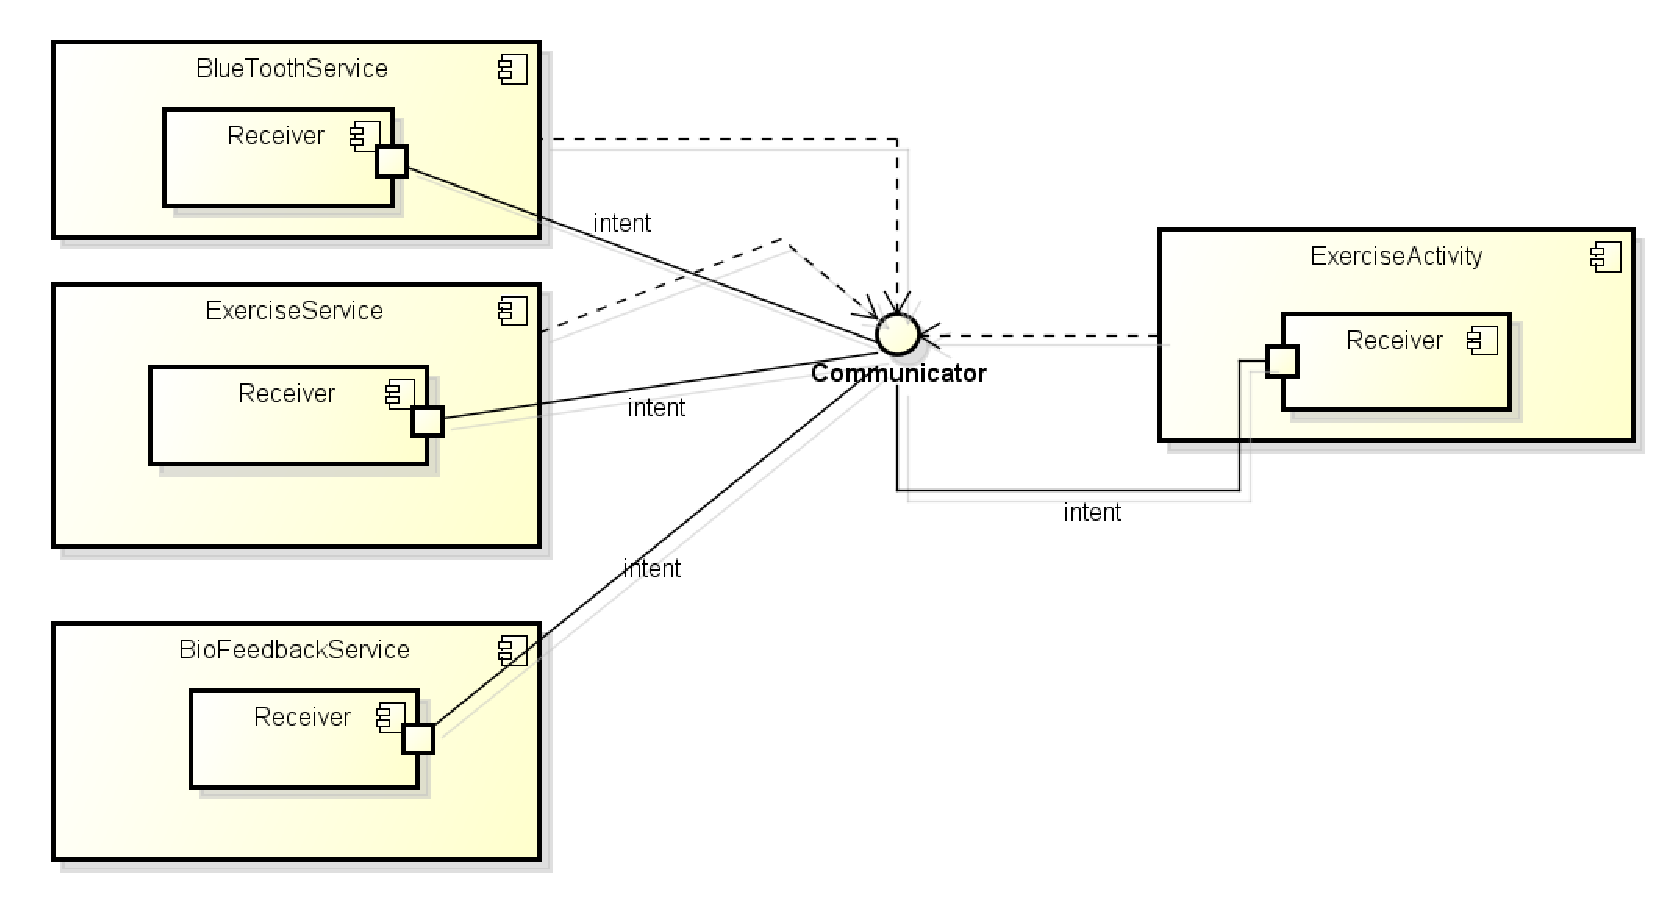
\includegraphics [keepaspectratio=true,scale=0.60]{figuras/diagramaComponentes.eps}
\caption{Componentes e sua comunicação via classe \textit{Communicator}}
\label{diagramaComponentes}
\end{figure}

A única exceção para essa comunicação indireta é a própria inicialização dos componentes. Todos os serviços precisam ser iniciados em algum lugar na aplicação, e o lugar óbvio para o fazer é no início da aplicação. Não tem porque iniciar os componentes enquanto o usuário não abrir a parte gráfica da aplicação, e por esse motivo os serviços são inicializados assim que a \textit{Activity} principal é criada, já que ela é o ponto de entrada da aplicação e-lastic. Muitos componentes podem ser o ponto de entrada em um aplicativo Android, mas neste caso específico a melhor escolha é a própria interface gráfica, representada pela \textit{Activity}. Desse modo a \textit{Activity} conhece os serviços a serem inicializados, porém não conhece seu comportamento e nem mesmo sua responsabilidade.

Essa comunicação por meio do LocalBroadcastManager funciona de maneira semelhante ao que vemos no padrão observador de orientação a objetos. Todos os ``eventos'' ou ``mensagens'' gerados em um componente/módulo são informados ao objeto exclusivo ao contexto do aplicativo, que por sua vez os entrega a quem se inscreveu para obtê-los. Uma diferença básica em relação a essa comparação é que no padrão observador, a interface gráfica geralmente conhece a classe de modelo na qual se inscreve para receber atualizações, e portanto existe uma relação unilateral fraca entre os objetos. Da forma implementada neste trabalho, cada objeto apenas conhece as mensagens que quer receber e como elas são formatadas mas não o componente que as envia, deixando as classes mais desacopladas. Entretanto, o resultado de uma análise de fator de acoplamento pode indicar um valor não tão pequeno devido a utilização da classe Communicator pelos demais componentes. Nessa arquitetura, é uma classe com alto acoplamento unilateral, pois, embora ela não conheça os componentes que receberão as mensagens, a maioria dos componentes a conhecem e a utilizam como ``mensageiro''. 

A Figura\ref{diagramaComponentes} é um diagrama de componentes que representa de forma gráfica a ideia básica da comunicação entre os componentes da aplicação e-lastic.

\begin{figure}[!htb]
\centering
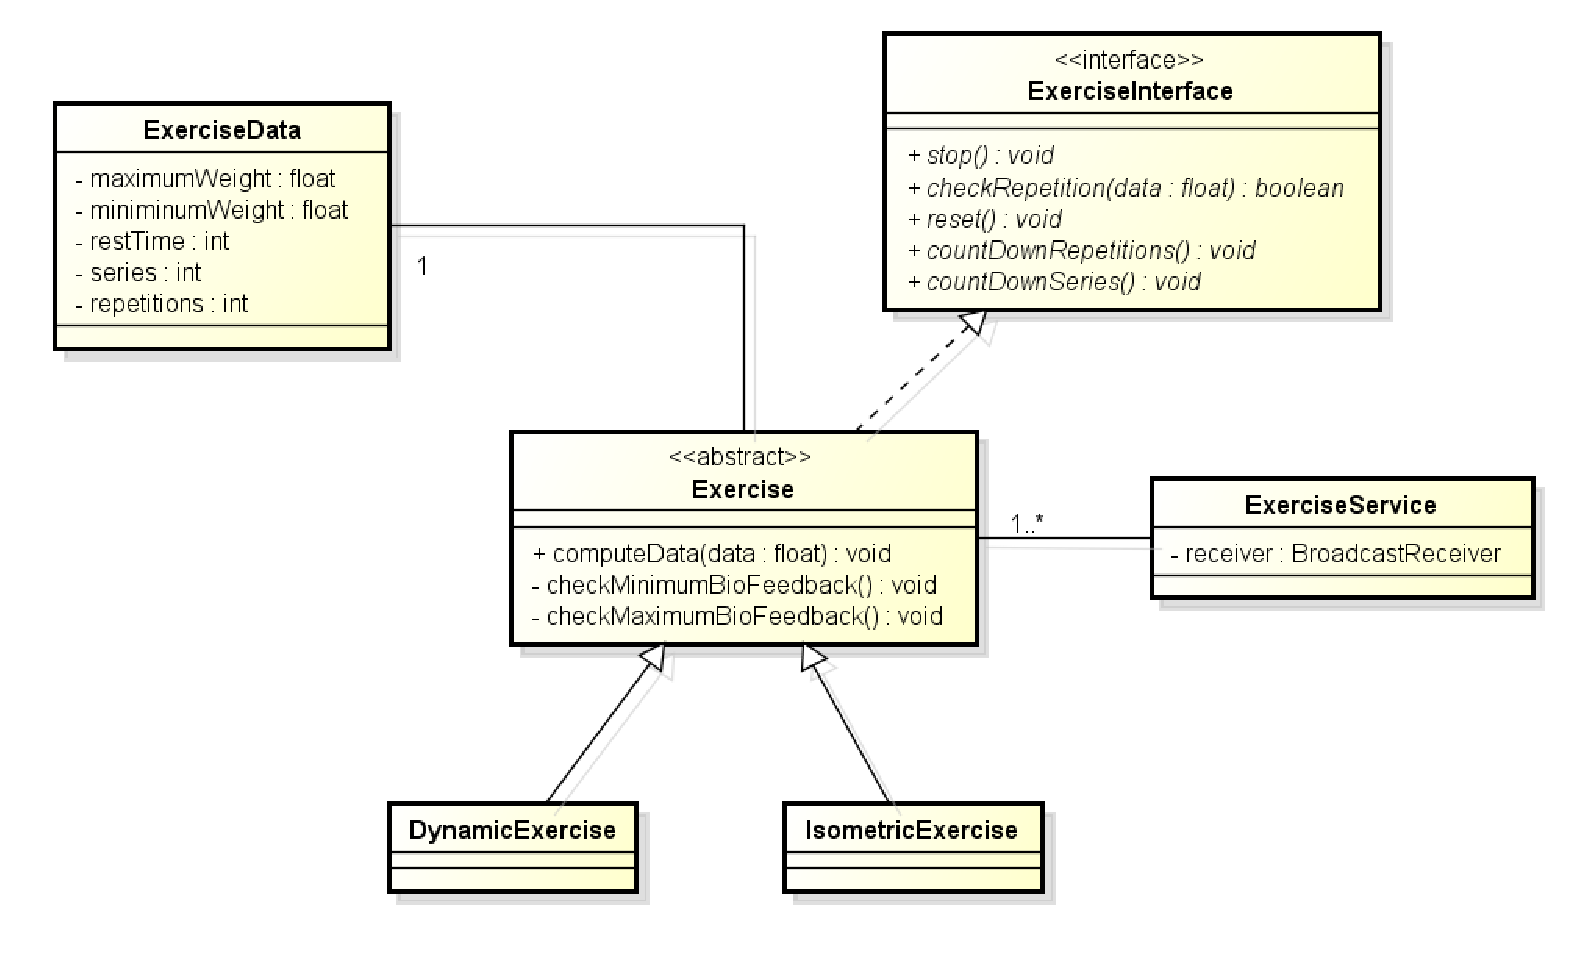
\includegraphics [keepaspectratio=true,scale=0.60]{figuras/diagramaExercicios.eps}
\caption{Principais classes dentro do módulo de exercício e suas relações}
\label{diagramaExercicios}
\end{figure}

Embora representado no diagrama de componentes como uma caixa apenas (\textit{ExerciseService}), o módulo de exercício contém a lógica da comunicação do componente via \textit{Communicator} e o gerenciamento do exercício em execução. É utilizada a generalização para que o \textit{service} tenha o mesmo comportamento independente do exercício em execução, e portanto as manipulações do exercício são feitas em cima de um objeto do tipo \textit{Exercise}, que é uma classe abstrata. A Figura~\ref{diagramaExercicios} contém um diagrama de classes para demonstrar a estrutura básica desse módulo.

\begin{figure}[!htb]
\centering
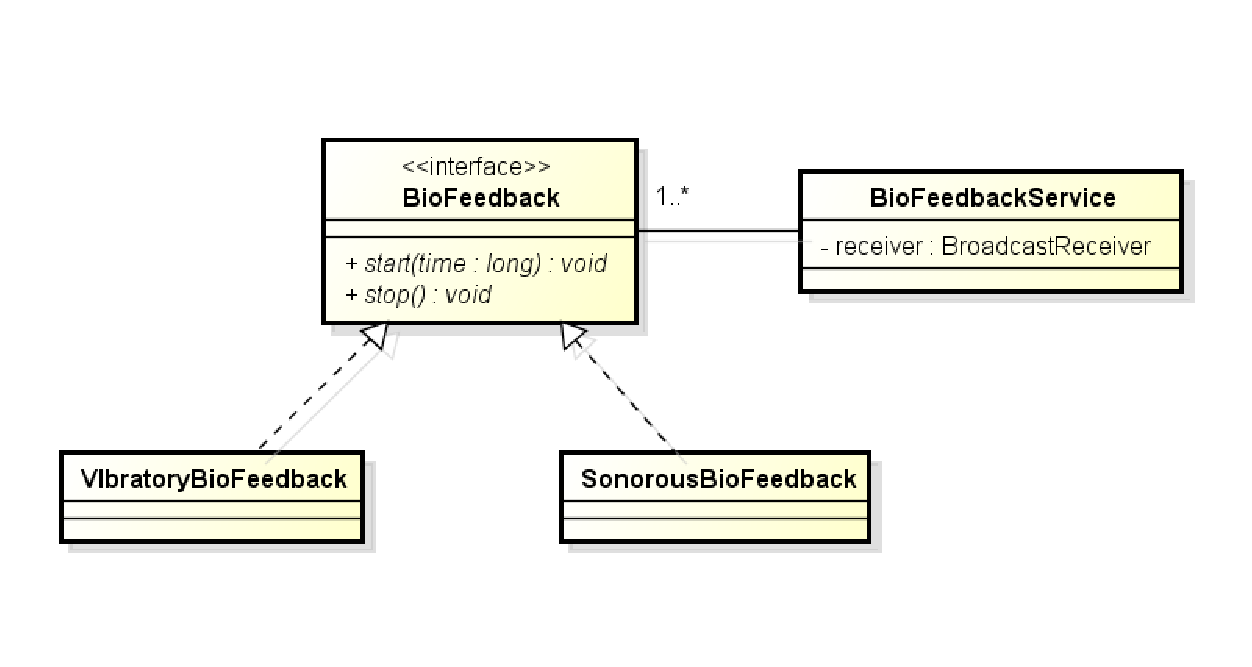
\includegraphics [keepaspectratio=true,scale=0.60]{figuras/diagramaBioFeedback.eps}
\caption{Principais classes dentro do módulo de \textit{biofeedback} e suas relações}
\label{diagramaBioFeedback}
\end{figure}

As classes internas do módulo de \textit{biofeedback} podem ser vistas na Figura~\ref{diagramaBioFeedback}. Também é utilizada uma generalização dos tipos de \textit{biofeedback} com a interface \textit{BioFeedback}, que deve ser implementada para criar um novo tipo de \textit{biofeedback}. Da mesma forma que o módulo de exercício, aqui também existe um \textit{service} que fica em segundo plano a espera de uma requisição de execução de \textit{biofeedback}. Em suma, ele fica em \textit{standby} até que algum pedaço da aplicação solicite que ele ative algum dos seus tipos de \textit{feedback}. Reunir essa função em um módulo específico da aplicação faz com que se possa ter controle de quais tipos de \textit{biofeedback} podem ser utilizados, e eles tem um acesso padrão independente do tipo, com a utilização do \textit{Communicator} e \textit{flags} que identificam que tipos de \textit{biofeedback} ativar. Tocar um som e vibrar o celular são feitos de formas completamente diferentes, e só a própria classe precisa saber como o fazer, sendo que o \textit{service} só conhece a interface de início e término e para ela não importa sua implementação. Com a implementação dessa forma, basta uma adição de uma linha de código no mapa de \textit{biofeedbacks} e a adição de uma \textit{flag}, além da implementação do novo \textit{biofeedback}, para que um novo tipo de \textit{biofeedback} esteja pronto para ser utilizado.

As explicações neste tópico tem como objetivo principal tentar demonstrar o tipo de comunicação entre as partes da aplicação e a modularização da mesma, justificando as principais decisões acerca da arquitetura e demonstrando a preocupação da equipe com manutenibilidade e princípios de design. Não serão explorados todos os detalhes da implementação da aplicação desenvolvida, sendo que isso será o alvo da segunda parte deste trabalho.